\documentclass[twoside]{book}

% Packages required by doxygen
\usepackage{fixltx2e}
\usepackage{calc}
\usepackage{doxygen}
\usepackage[export]{adjustbox} % also loads graphicx
\usepackage{graphicx}
\usepackage[utf8]{inputenc}
\usepackage{makeidx}
\usepackage{multicol}
\usepackage{multirow}
\PassOptionsToPackage{warn}{textcomp}
\usepackage{textcomp}
\usepackage[nointegrals]{wasysym}
\usepackage[table]{xcolor}

% Font selection
\usepackage[T1]{fontenc}
\usepackage[scaled=.90]{helvet}
\usepackage{courier}
\usepackage{amssymb}
\usepackage{sectsty}
\renewcommand{\familydefault}{\sfdefault}
\allsectionsfont{%
  \fontseries{bc}\selectfont%
  \color{darkgray}%
}
\renewcommand{\DoxyLabelFont}{%
  \fontseries{bc}\selectfont%
  \color{darkgray}%
}
\newcommand{\+}{\discretionary{\mbox{\scriptsize$\hookleftarrow$}}{}{}}

% Page & text layout
\usepackage{geometry}
\geometry{%
  a4paper,%
  top=2.5cm,%
  bottom=2.5cm,%
  left=2.5cm,%
  right=2.5cm%
}
\tolerance=750
\hfuzz=15pt
\hbadness=750
\setlength{\emergencystretch}{15pt}
\setlength{\parindent}{0cm}
\setlength{\parskip}{3ex plus 2ex minus 2ex}
\makeatletter
\renewcommand{\paragraph}{%
  \@startsection{paragraph}{4}{0ex}{-1.0ex}{1.0ex}{%
    \normalfont\normalsize\bfseries\SS@parafont%
  }%
}
\renewcommand{\subparagraph}{%
  \@startsection{subparagraph}{5}{0ex}{-1.0ex}{1.0ex}{%
    \normalfont\normalsize\bfseries\SS@subparafont%
  }%
}
\makeatother

% Headers & footers
\usepackage{fancyhdr}
\pagestyle{fancyplain}
\fancyhead[LE]{\fancyplain{}{\bfseries\thepage}}
\fancyhead[CE]{\fancyplain{}{}}
\fancyhead[RE]{\fancyplain{}{\bfseries\leftmark}}
\fancyhead[LO]{\fancyplain{}{\bfseries\rightmark}}
\fancyhead[CO]{\fancyplain{}{}}
\fancyhead[RO]{\fancyplain{}{\bfseries\thepage}}
\fancyfoot[LE]{\fancyplain{}{}}
\fancyfoot[CE]{\fancyplain{}{}}
\fancyfoot[RE]{\fancyplain{}{\bfseries\scriptsize Generated by Doxygen }}
\fancyfoot[LO]{\fancyplain{}{\bfseries\scriptsize Generated by Doxygen }}
\fancyfoot[CO]{\fancyplain{}{}}
\fancyfoot[RO]{\fancyplain{}{}}
\renewcommand{\footrulewidth}{0.4pt}
\renewcommand{\chaptermark}[1]{%
  \markboth{#1}{}%
}
\renewcommand{\sectionmark}[1]{%
  \markright{\thesection\ #1}%
}

% Indices & bibliography
\usepackage{natbib}
\usepackage[titles]{tocloft}
\setcounter{tocdepth}{3}
\setcounter{secnumdepth}{5}
\makeindex

% Hyperlinks (required, but should be loaded last)
\usepackage{ifpdf}
\ifpdf
  \usepackage[pdftex,pagebackref=true]{hyperref}
\else
  \usepackage[ps2pdf,pagebackref=true]{hyperref}
\fi
\hypersetup{%
  colorlinks=true,%
  linkcolor=blue,%
  citecolor=blue,%
  unicode%
}

% Custom commands
\newcommand{\clearemptydoublepage}{%
  \newpage{\pagestyle{empty}\cleardoublepage}%
}

\usepackage{caption}
\captionsetup{labelsep=space,justification=centering,font={bf},singlelinecheck=off,skip=4pt,position=top}

%===== C O N T E N T S =====

\begin{document}

% Titlepage & ToC
\hypersetup{pageanchor=false,
             bookmarksnumbered=true,
             pdfencoding=unicode
            }
\pagenumbering{roman}
\begin{titlepage}
\vspace*{7cm}
\begin{center}%
{\Large Laser Scanner infoscreen \\[1ex]\large 1.\+0 }\\
\vspace*{1cm}
{\large Generated by Doxygen 1.8.11}\\
\end{center}
\end{titlepage}
\clearemptydoublepage
\tableofcontents
\clearemptydoublepage
\pagenumbering{arabic}
\hypersetup{pageanchor=true}

%--- Begin generated contents ---
\chapter{Class Index}
\section{Class List}
Here are the classes, structs, unions and interfaces with brief descriptions\+:\begin{DoxyCompactList}
\item\contentsline{section}{\hyperlink{structpoi__t}{poi\+\_\+t} \\*Person of interest }{\pageref{structpoi__t}}{}
\end{DoxyCompactList}

\chapter{File Index}
\section{File List}
Here is a list of all documented files with brief descriptions\+:\begin{DoxyCompactList}
\item\contentsline{section}{include/\hyperlink{laser__objects_8hpp}{laser\+\_\+objects.\+hpp} }{\pageref{laser__objects_8hpp}}{}
\item\contentsline{section}{include/\hyperlink{scanner__gestures_8h}{scanner\+\_\+gestures.\+h} }{\pageref{scanner__gestures_8h}}{}
\item\contentsline{section}{src/\hyperlink{control__tcp__socket_8cpp}{control\+\_\+tcp\+\_\+socket.\+cpp} }{\pageref{control__tcp__socket_8cpp}}{}
\item\contentsline{section}{src/\hyperlink{gesture__control_8cpp}{gesture\+\_\+control.\+cpp} \\*Node that handles gesture tracking and associated topics }{\pageref{gesture__control_8cpp}}{}
\item\contentsline{section}{src/\hyperlink{laser__objects_8cpp}{laser\+\_\+objects.\+cpp} \\*Implementation of object tracking }{\pageref{laser__objects_8cpp}}{}
\item\contentsline{section}{src/\hyperlink{measure__biometrics_8cpp}{measure\+\_\+biometrics.\+cpp} \\*A naive implementation of biometrics measurements }{\pageref{measure__biometrics_8cpp}}{}
\item\contentsline{section}{src/\hyperlink{scanner__gestures_8cpp}{scanner\+\_\+gestures.\+cpp} }{\pageref{scanner__gestures_8cpp}}{}
\item\contentsline{section}{src/\hyperlink{track__objects__client_8cpp}{track\+\_\+objects\+\_\+client.\+cpp} \\*R\+OS Client node of object tracker }{\pageref{track__objects__client_8cpp}}{}
\item\contentsline{section}{src/\hyperlink{track__objects__server_8cpp}{track\+\_\+objects\+\_\+server.\+cpp} \\*R\+OS Service node of object tracker }{\pageref{track__objects__server_8cpp}}{}
\end{DoxyCompactList}

\chapter{Class Documentation}
\hypertarget{structpoi__t}{}\section{poi\+\_\+t Struct Reference}
\label{structpoi__t}\index{poi\+\_\+t@{poi\+\_\+t}}


position of the PoI in polar coordinates  


\subsection*{Public Attributes}
\begin{DoxyCompactItemize}
\item 
float \hyperlink{structpoi__t_ae5f9ca22bbe2f78476ad6d08bc31a231}{poi\+\_\+range}
\item 
float \hyperlink{structpoi__t_a59b58f432e793217c33691e9c8b921b7}{poi\+\_\+angle}
\end{DoxyCompactItemize}


\subsection{Detailed Description}
position of the PoI in polar coordinates 

Contains range and angle data of the object the system is currently tracking. 

\subsection{Member Data Documentation}
\index{poi\+\_\+t@{poi\+\_\+t}!poi\+\_\+angle@{poi\+\_\+angle}}
\index{poi\+\_\+angle@{poi\+\_\+angle}!poi\+\_\+t@{poi\+\_\+t}}
\subsubsection[{\texorpdfstring{poi\+\_\+angle}{poi_angle}}]{\setlength{\rightskip}{0pt plus 5cm}float poi\+\_\+t\+::poi\+\_\+angle}\hypertarget{structpoi__t_a59b58f432e793217c33691e9c8b921b7}{}\label{structpoi__t_a59b58f432e793217c33691e9c8b921b7}
angle of the PoI in radians. 0 is directly at the front. \index{poi\+\_\+t@{poi\+\_\+t}!poi\+\_\+range@{poi\+\_\+range}}
\index{poi\+\_\+range@{poi\+\_\+range}!poi\+\_\+t@{poi\+\_\+t}}
\subsubsection[{\texorpdfstring{poi\+\_\+range}{poi_range}}]{\setlength{\rightskip}{0pt plus 5cm}float poi\+\_\+t\+::poi\+\_\+range}\hypertarget{structpoi__t_ae5f9ca22bbe2f78476ad6d08bc31a231}{}\label{structpoi__t_ae5f9ca22bbe2f78476ad6d08bc31a231}
range of the PoI in metres 

The documentation for this struct was generated from the following files\+:\begin{DoxyCompactItemize}
\item 
src/\hyperlink{gesture__control_8cpp}{gesture\+\_\+control.\+cpp}\item 
src/\hyperlink{track__objects__client_8cpp}{track\+\_\+objects\+\_\+client.\+cpp}\end{DoxyCompactItemize}

\chapter{File Documentation}
\hypertarget{laser__objects_8hpp}{}\section{include/laser\+\_\+objects.hpp File Reference}
\label{laser__objects_8hpp}\index{include/laser\+\_\+objects.\+hpp@{include/laser\+\_\+objects.\+hpp}}
{\ttfamily \#include $<$armadillo$>$}\\*
Include dependency graph for laser\+\_\+objects.\+hpp\+:\nopagebreak
\begin{figure}[H]
\begin{center}
\leavevmode
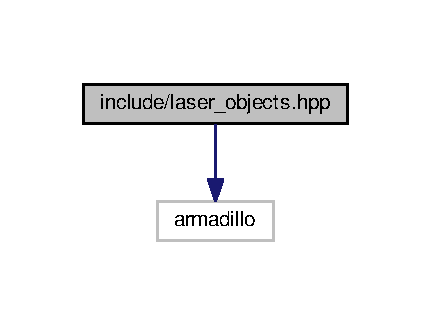
\includegraphics[width=207pt]{laser__objects_8hpp__incl}
\end{center}
\end{figure}
This graph shows which files directly or indirectly include this file\+:\nopagebreak
\begin{figure}[H]
\begin{center}
\leavevmode
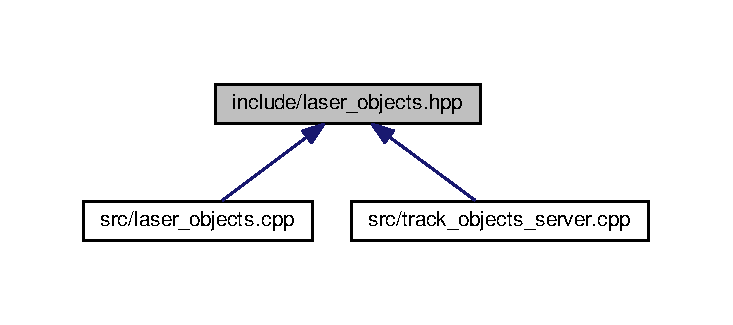
\includegraphics[width=350pt]{laser__objects_8hpp__dep__incl}
\end{center}
\end{figure}
\subsection*{Classes}
\begin{DoxyCompactItemize}
\item 
class \hyperlink{classlaser__object__t}{laser\+\_\+object\+\_\+t}
\begin{DoxyCompactList}\small\item\em An instance of tracked object. \end{DoxyCompactList}\item 
class \hyperlink{classlaser__objects}{laser\+\_\+objects}
\begin{DoxyCompactList}\small\item\em A repository for \hyperlink{classlaser__object__t}{laser\+\_\+object\+\_\+t}\textquotesingle{}s. \end{DoxyCompactList}\end{DoxyCompactItemize}

\hypertarget{scanner__gestures_8h}{}\section{include/scanner\+\_\+gestures.h File Reference}
\label{scanner__gestures_8h}\index{include/scanner\+\_\+gestures.\+h@{include/scanner\+\_\+gestures.\+h}}
{\ttfamily \#include \char`\"{}ros/ros.\+h\char`\"{}}\\*
Include dependency graph for scanner\+\_\+gestures.\+h\+:\nopagebreak
\begin{figure}[H]
\begin{center}
\leavevmode
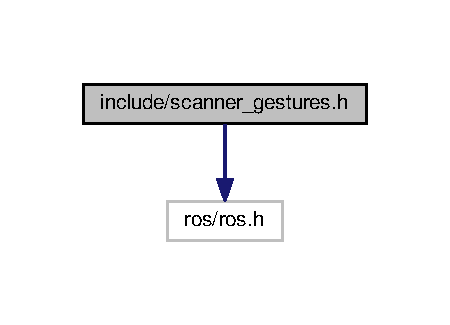
\includegraphics[width=216pt]{scanner__gestures_8h__incl}
\end{center}
\end{figure}
This graph shows which files directly or indirectly include this file\+:\nopagebreak
\begin{figure}[H]
\begin{center}
\leavevmode
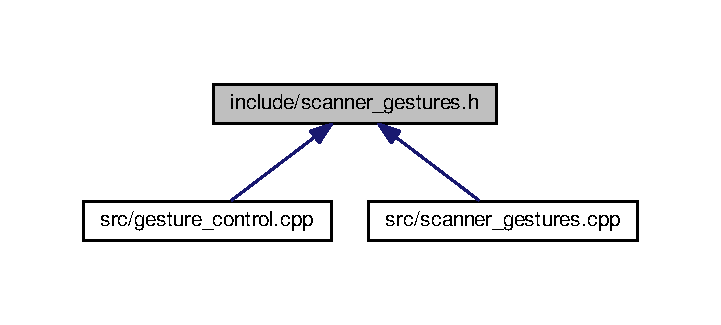
\includegraphics[width=346pt]{scanner__gestures_8h__dep__incl}
\end{center}
\end{figure}

\hypertarget{control__tcp__socket_8cpp}{}\section{src/control\+\_\+tcp\+\_\+socket.cpp File Reference}
\label{control__tcp__socket_8cpp}\index{src/control\+\_\+tcp\+\_\+socket.\+cpp@{src/control\+\_\+tcp\+\_\+socket.\+cpp}}
{\ttfamily \#include \char`\"{}ros/ros.\+h\char`\"{}}\\*
{\ttfamily \#include \char`\"{}laser\+\_\+scanner\+\_\+infoscreen/external\+\_\+control.\+h\char`\"{}}\\*
{\ttfamily \#include $<$iostream$>$}\\*
{\ttfamily \#include $<$string.\+h$>$}\\*
{\ttfamily \#include $<$sys/types.\+h$>$}\\*
{\ttfamily \#include $<$netinet/in.\+h$>$}\\*
{\ttfamily \#include $<$arpa/inet.\+h$>$}\\*
{\ttfamily \#include $<$stdlib.\+h$>$}\\*
{\ttfamily \#include $<$unistd.\+h$>$}\\*
{\ttfamily \#include $<$netdb.\+h$>$}\\*
Include dependency graph for control\+\_\+tcp\+\_\+socket.\+cpp\+:\nopagebreak
\begin{figure}[H]
\begin{center}
\leavevmode
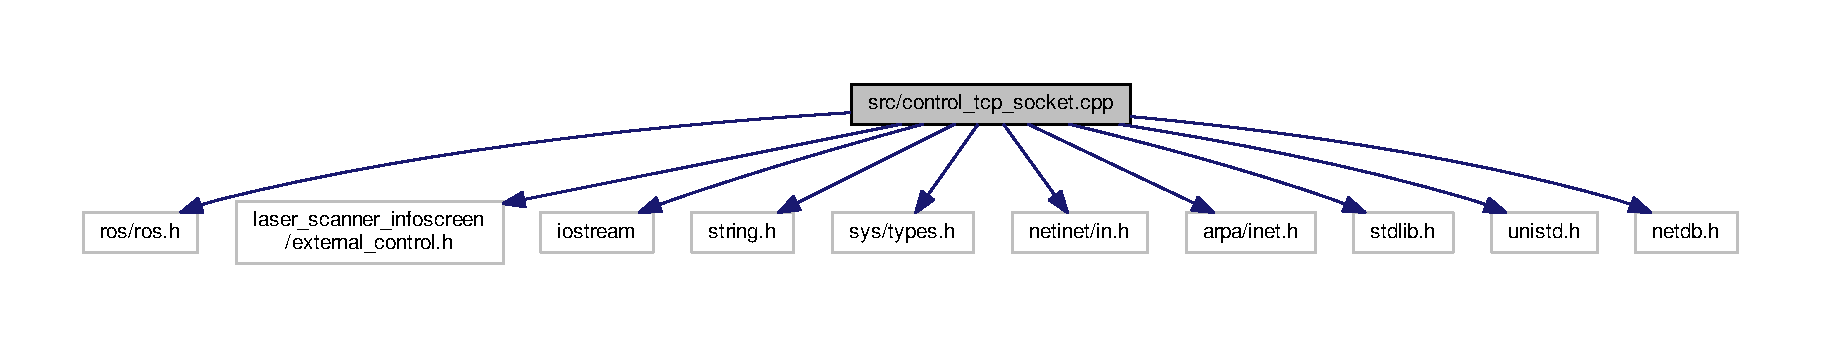
\includegraphics[width=350pt]{control__tcp__socket_8cpp__incl}
\end{center}
\end{figure}
\subsection*{Macros}
\begin{DoxyCompactItemize}
\item 
\#define \hyperlink{control__tcp__socket_8cpp_a22cfe843bbfa92fae8f2e4f0692ece94}{C\+H\+A\+R\+\_\+\+B\+U\+F\+F\+E\+R\+\_\+\+S\+I\+ZE}~512
\item 
\#define \hyperlink{control__tcp__socket_8cpp_aa6cecb8c404241c624e83aee8a3979d2}{S\+E\+R\+V\+E\+R\+\_\+\+A\+D\+D\+R\+E\+SS}~localhost
\end{DoxyCompactItemize}
\subsection*{Functions}
\begin{DoxyCompactItemize}
\item 
void \hyperlink{control__tcp__socket_8cpp_ae394a55d4227c16bca1b6e1ba6a5e8b4}{tcp\+\_\+message\+\_\+callback} (const laser\+\_\+scanner\+\_\+infoscreen\+::external\+\_\+control\+::\+Const\+Ptr \&msg)
\begin{DoxyCompactList}\small\item\em external\+\_\+control callback function. \end{DoxyCompactList}\item 
int \hyperlink{control__tcp__socket_8cpp_a3c04138a5bfe5d72780bb7e82a18e627}{main} (int argc, char $\ast$$\ast$argv)
\end{DoxyCompactItemize}


\subsection{Detailed Description}
R\+OS node for the running infoscreen. Subscribes to the \textquotesingle{}/external\+\_\+control\textquotesingle{} topic, receives, parses and send messages on the T\+CP socket for the G\+UI. \begin{DoxySeeAlso}{See also}
$<$track\+\_\+objects\+\_\+client$>$ 
\end{DoxySeeAlso}


\subsection{Macro Definition Documentation}
\index{control\+\_\+tcp\+\_\+socket.\+cpp@{control\+\_\+tcp\+\_\+socket.\+cpp}!C\+H\+A\+R\+\_\+\+B\+U\+F\+F\+E\+R\+\_\+\+S\+I\+ZE@{C\+H\+A\+R\+\_\+\+B\+U\+F\+F\+E\+R\+\_\+\+S\+I\+ZE}}
\index{C\+H\+A\+R\+\_\+\+B\+U\+F\+F\+E\+R\+\_\+\+S\+I\+ZE@{C\+H\+A\+R\+\_\+\+B\+U\+F\+F\+E\+R\+\_\+\+S\+I\+ZE}!control\+\_\+tcp\+\_\+socket.\+cpp@{control\+\_\+tcp\+\_\+socket.\+cpp}}
\subsubsection[{\texorpdfstring{C\+H\+A\+R\+\_\+\+B\+U\+F\+F\+E\+R\+\_\+\+S\+I\+ZE}{CHAR_BUFFER_SIZE}}]{\setlength{\rightskip}{0pt plus 5cm}\#define C\+H\+A\+R\+\_\+\+B\+U\+F\+F\+E\+R\+\_\+\+S\+I\+ZE~512}\hypertarget{control__tcp__socket_8cpp_a22cfe843bbfa92fae8f2e4f0692ece94}{}\label{control__tcp__socket_8cpp_a22cfe843bbfa92fae8f2e4f0692ece94}
Size of the buffer used by the T\+CP node. \index{control\+\_\+tcp\+\_\+socket.\+cpp@{control\+\_\+tcp\+\_\+socket.\+cpp}!S\+E\+R\+V\+E\+R\+\_\+\+A\+D\+D\+R\+E\+SS@{S\+E\+R\+V\+E\+R\+\_\+\+A\+D\+D\+R\+E\+SS}}
\index{S\+E\+R\+V\+E\+R\+\_\+\+A\+D\+D\+R\+E\+SS@{S\+E\+R\+V\+E\+R\+\_\+\+A\+D\+D\+R\+E\+SS}!control\+\_\+tcp\+\_\+socket.\+cpp@{control\+\_\+tcp\+\_\+socket.\+cpp}}
\subsubsection[{\texorpdfstring{S\+E\+R\+V\+E\+R\+\_\+\+A\+D\+D\+R\+E\+SS}{SERVER_ADDRESS}}]{\setlength{\rightskip}{0pt plus 5cm}\#define S\+E\+R\+V\+E\+R\+\_\+\+A\+D\+D\+R\+E\+SS~localhost}\hypertarget{control__tcp__socket_8cpp_aa6cecb8c404241c624e83aee8a3979d2}{}\label{control__tcp__socket_8cpp_aa6cecb8c404241c624e83aee8a3979d2}
Address of the T\+CP node. Currently runs only one localhost. 

\subsection{Function Documentation}
\index{control\+\_\+tcp\+\_\+socket.\+cpp@{control\+\_\+tcp\+\_\+socket.\+cpp}!main@{main}}
\index{main@{main}!control\+\_\+tcp\+\_\+socket.\+cpp@{control\+\_\+tcp\+\_\+socket.\+cpp}}
\subsubsection[{\texorpdfstring{main(int argc, char $\ast$$\ast$argv)}{main(int argc, char **argv)}}]{\setlength{\rightskip}{0pt plus 5cm}int main (
\begin{DoxyParamCaption}
\item[{int}]{argc, }
\item[{char $\ast$$\ast$}]{argv}
\end{DoxyParamCaption}
)}\hypertarget{control__tcp__socket_8cpp_a3c04138a5bfe5d72780bb7e82a18e627}{}\label{control__tcp__socket_8cpp_a3c04138a5bfe5d72780bb7e82a18e627}
Main function of the node Main function of the node. Creates socket, binds it and sets R\+OS to run. Handles cleanup.

Node currently uses port 2259 as it is free per \href{https://www.iana.org/assignments/service-names-port-numbers/service-names-port-numbers.xhtm}{\tt https\+://www.\+iana.\+org/assignments/service-\/names-\/port-\/numbers/service-\/names-\/port-\/numbers.\+xhtm} \index{control\+\_\+tcp\+\_\+socket.\+cpp@{control\+\_\+tcp\+\_\+socket.\+cpp}!tcp\+\_\+message\+\_\+callback@{tcp\+\_\+message\+\_\+callback}}
\index{tcp\+\_\+message\+\_\+callback@{tcp\+\_\+message\+\_\+callback}!control\+\_\+tcp\+\_\+socket.\+cpp@{control\+\_\+tcp\+\_\+socket.\+cpp}}
\subsubsection[{\texorpdfstring{tcp\+\_\+message\+\_\+callback(const laser\+\_\+scanner\+\_\+infoscreen\+::external\+\_\+control\+::\+Const\+Ptr \&msg)}{tcp_message_callback(const laser_scanner_infoscreen::external_control::ConstPtr &msg)}}]{\setlength{\rightskip}{0pt plus 5cm}void tcp\+\_\+message\+\_\+callback (
\begin{DoxyParamCaption}
\item[{const laser\+\_\+scanner\+\_\+infoscreen\+::external\+\_\+control\+::\+Const\+Ptr \&}]{msg}
\end{DoxyParamCaption}
)}\hypertarget{control__tcp__socket_8cpp_ae394a55d4227c16bca1b6e1ba6a5e8b4}{}\label{control__tcp__socket_8cpp_ae394a55d4227c16bca1b6e1ba6a5e8b4}


external\+\_\+control callback function. 

A callback function of topic external\+\_\+control. Parses and send message by T\+CP. 
\begin{DoxyParams}{Parameters}
{\em msg} & topic message outlined in msg/external\+\_\+control.\+msg \\
\hline
\end{DoxyParams}

\hypertarget{gesture__control_8cpp}{}\section{src/gesture\+\_\+control.cpp File Reference}
\label{gesture__control_8cpp}\index{src/gesture\+\_\+control.\+cpp@{src/gesture\+\_\+control.\+cpp}}


Node that handles gesture tracking and associated topics.  


{\ttfamily \#include \char`\"{}ros/ros.\+h\char`\"{}}\\*
{\ttfamily \#include \char`\"{}laser\+\_\+scanner\+\_\+infoscreen/servo\+\_\+control.\+h\char`\"{}}\\*
{\ttfamily \#include \char`\"{}laser\+\_\+scanner\+\_\+infoscreen/servo\+\_\+feedback.\+h\char`\"{}}\\*
{\ttfamily \#include \char`\"{}laser\+\_\+scanner\+\_\+infoscreen/external\+\_\+control.\+h\char`\"{}}\\*
{\ttfamily \#include \char`\"{}scanner\+\_\+gestures.\+h\char`\"{}}\\*
{\ttfamily \#include \char`\"{}laser\+\_\+scanner\+\_\+infoscreen/gesture\+\_\+call.\+h\char`\"{}}\\*
{\ttfamily \#include \char`\"{}sensor\+\_\+msgs/\+Laser\+Scan.\+h\char`\"{}}\\*
{\ttfamily \#include $<$cstdlib$>$}\\*
{\ttfamily \#include $<$cmath$>$}\\*
{\ttfamily \#include $<$visualization\+\_\+msgs/\+Marker.\+h$>$}\\*
{\ttfamily \#include $<$string$>$}\\*
Include dependency graph for gesture\+\_\+control.\+cpp\+:\nopagebreak
\begin{figure}[H]
\begin{center}
\leavevmode
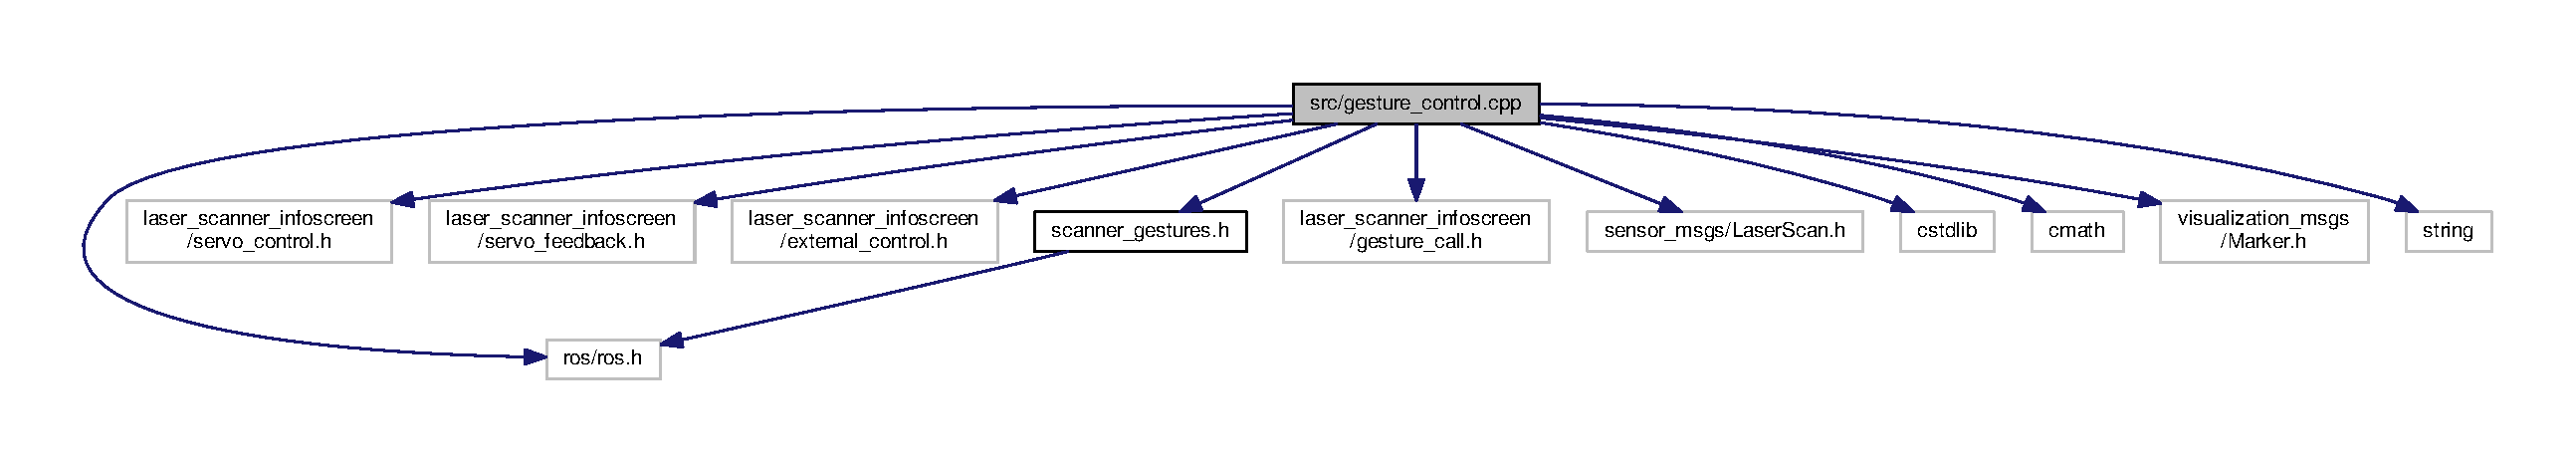
\includegraphics[width=350pt]{gesture__control_8cpp__incl}
\end{center}
\end{figure}
\subsection*{Classes}
\begin{DoxyCompactItemize}
\item 
struct \hyperlink{structpoi__t}{poi\+\_\+t}
\begin{DoxyCompactList}\small\item\em position of the PoI in polar coordinates \end{DoxyCompactList}\item 
struct \hyperlink{structservo__t}{servo\+\_\+t}
\begin{DoxyCompactList}\small\item\em Lock for the servo control (e.\+g. busy with biometrics) \end{DoxyCompactList}\end{DoxyCompactItemize}
\subsection*{Macros}
\begin{DoxyCompactItemize}
\item 
\#define \hyperlink{gesture__control_8cpp_ae50e2e14bc27c23e04b985bd48ebb83b}{timeout\+\_\+limit}~4
\begin{DoxyCompactList}\small\item\em Seconds after old gesture timeouts. \end{DoxyCompactList}\item 
\#define \hyperlink{gesture__control_8cpp_ab013d51a86bf4715a1c261218605c915}{gesture\+\_\+score\+\_\+threshold}~1.\+0f
\item 
\#define \hyperlink{gesture__control_8cpp_a652fa32c4482bb0d3805c3c5f5900af5}{servo\+\_\+speed\+\_\+const}~5235
\item 
\#define \hyperlink{gesture__control_8cpp_aafa72341f1113b0939af781b7d63770d}{servo\+\_\+loop\+\_\+len}~5
\begin{DoxyCompactList}\small\item\em Length of servo idle loop. \end{DoxyCompactList}\end{DoxyCompactItemize}
\subsection*{Functions}
\begin{DoxyCompactItemize}
\item 
void \hyperlink{gesture__control_8cpp_adbf76bdb1d65ea9f9d44ec58eb40d877}{gestures\+\_\+callback} (const sensor\+\_\+msgs\+::\+Laser\+Scan\+::\+Const\+Ptr \&scan)
\begin{DoxyCompactList}\small\item\em if enables, parses Laser\+Scan messages and send them to the gesture tracker. \end{DoxyCompactList}\item 
void \hyperlink{gesture__control_8cpp_ab4546fc84eafe7c48c81b8f28c5077c1}{control\+\_\+callback} (const laser\+\_\+scanner\+\_\+infoscreen\+::gesture\+\_\+call \&msg)
\begin{DoxyCompactList}\small\item\em handles control messages from /gesture\+\_\+control topic \end{DoxyCompactList}\item 
void \hyperlink{gesture__control_8cpp_a272dea7f151f9bf75131542422903056}{servo\+\_\+feedback\+\_\+callback} (const laser\+\_\+scanner\+\_\+infoscreen\+::servo\+\_\+feedback \&msg)
\begin{DoxyCompactList}\small\item\em servo controller callback to release servo lock. \end{DoxyCompactList}\item 
int \hyperlink{gesture__control_8cpp_a3c04138a5bfe5d72780bb7e82a18e627}{main} (int argc, char $\ast$$\ast$argv)
\end{DoxyCompactItemize}
\subsection*{Variables}
\begin{DoxyCompactItemize}
\item 
static std\+::vector$<$ float $>$ \hyperlink{gesture__control_8cpp_ad8662d30f3440d45487607002371a735}{sensor\+\_\+pos} = \{0.\+0,-\/0.\+22,0.\+72\}\hypertarget{gesture__control_8cpp_ad8662d30f3440d45487607002371a735}{}\label{gesture__control_8cpp_ad8662d30f3440d45487607002371a735}

\begin{DoxyCompactList}\small\item\em Offset of the upper sensor in the relation of lower sensor in \{x,y,z\}. \end{DoxyCompactList}\item 
int \hyperlink{gesture__control_8cpp_a2ac8bc219bf895e4a3cdd514c1de6ec4}{loop\+\_\+count} = 0
\begin{DoxyCompactList}\small\item\em Loop counter fo the servo control. \end{DoxyCompactList}\item 
static Scanner\+\_\+gestures $\ast$ \hyperlink{gesture__control_8cpp_a6565562c39be7f8f9a538a9a216a28cf}{gestures}\hypertarget{gesture__control_8cpp_a6565562c39be7f8f9a538a9a216a28cf}{}\label{gesture__control_8cpp_a6565562c39be7f8f9a538a9a216a28cf}

\begin{DoxyCompactList}\small\item\em Global pointer to Scanner\+\_\+gestures object. \end{DoxyCompactList}\item 
static ros\+::\+Node\+Handle $\ast$ \hyperlink{gesture__control_8cpp_a8c9e9fe63fc6db914caeb21d95be5ca0}{node\+\_\+pointer}\hypertarget{gesture__control_8cpp_a8c9e9fe63fc6db914caeb21d95be5ca0}{}\label{gesture__control_8cpp_a8c9e9fe63fc6db914caeb21d95be5ca0}

\begin{DoxyCompactList}\small\item\em Global pointer to ros\+::\+Node\+Handle object. \end{DoxyCompactList}\item 
ros\+::\+Publisher $\ast$ \hyperlink{gesture__control_8cpp_a63b0cea48d2da7a328302aee063e57b9}{marker\+\_\+pub\+\_\+pointer}\hypertarget{gesture__control_8cpp_a63b0cea48d2da7a328302aee063e57b9}{}\label{gesture__control_8cpp_a63b0cea48d2da7a328302aee063e57b9}

\begin{DoxyCompactList}\small\item\em Global pointer to rviz marker object. \end{DoxyCompactList}\item 
ros\+::\+Publisher $\ast$ \hyperlink{gesture__control_8cpp_ad7c4130fa2a9b5b52c9cc9762accfe31}{servo\+\_\+control\+\_\+pointer}\hypertarget{gesture__control_8cpp_ad7c4130fa2a9b5b52c9cc9762accfe31}{}\label{gesture__control_8cpp_ad7c4130fa2a9b5b52c9cc9762accfe31}

\begin{DoxyCompactList}\small\item\em Global pointer to \textquotesingle{}servo\+\_\+control\textquotesingle{} publisher. \end{DoxyCompactList}\item 
ros\+::\+Subscriber $\ast$ \hyperlink{gesture__control_8cpp_a25374abed3f304c24bfe5098b954d442}{gesture\+\_\+control\+\_\+pointer}\hypertarget{gesture__control_8cpp_a25374abed3f304c24bfe5098b954d442}{}\label{gesture__control_8cpp_a25374abed3f304c24bfe5098b954d442}

\begin{DoxyCompactList}\small\item\em Global pointer to \textquotesingle{}gestures\+\_\+control\textquotesingle{} subscriber. \end{DoxyCompactList}\item 
ros\+::\+Publisher $\ast$ \hyperlink{gesture__control_8cpp_a95ade72c9341fa47411a2314df6d9c0c}{external\+\_\+control\+\_\+pointer}\hypertarget{gesture__control_8cpp_a95ade72c9341fa47411a2314df6d9c0c}{}\label{gesture__control_8cpp_a95ade72c9341fa47411a2314df6d9c0c}

\begin{DoxyCompactList}\small\item\em Global pointer to \textquotesingle{}external\+\_\+control\textquotesingle{} publisher. Used to relay commands to external applications. \end{DoxyCompactList}\item 
static ros\+::\+Time \hyperlink{gesture__control_8cpp_a8bc0d59633fb23785a6dc267a7cb0326}{timelock}\hypertarget{gesture__control_8cpp_a8bc0d59633fb23785a6dc267a7cb0326}{}\label{gesture__control_8cpp_a8bc0d59633fb23785a6dc267a7cb0326}

\begin{DoxyCompactList}\small\item\em Global variable of last detected gesture timestamp. \end{DoxyCompactList}\end{DoxyCompactItemize}


\subsection{Detailed Description}
Node that handles gesture tracking and associated topics. 

\begin{DoxySeeAlso}{See also}
scanner\+\_\+gestures 

$<$track\+\_\+objects\+\_\+client$>$ 
\end{DoxySeeAlso}


\subsection{Macro Definition Documentation}
\index{gesture\+\_\+control.\+cpp@{gesture\+\_\+control.\+cpp}!gesture\+\_\+score\+\_\+threshold@{gesture\+\_\+score\+\_\+threshold}}
\index{gesture\+\_\+score\+\_\+threshold@{gesture\+\_\+score\+\_\+threshold}!gesture\+\_\+control.\+cpp@{gesture\+\_\+control.\+cpp}}
\subsubsection[{\texorpdfstring{gesture\+\_\+score\+\_\+threshold}{gesture_score_threshold}}]{\setlength{\rightskip}{0pt plus 5cm}\#define gesture\+\_\+score\+\_\+threshold~1.\+0f}\hypertarget{gesture__control_8cpp_ab013d51a86bf4715a1c261218605c915}{}\label{gesture__control_8cpp_ab013d51a86bf4715a1c261218605c915}
A score after which gesture is confirmed. Bigger is less likely \index{gesture\+\_\+control.\+cpp@{gesture\+\_\+control.\+cpp}!servo\+\_\+loop\+\_\+len@{servo\+\_\+loop\+\_\+len}}
\index{servo\+\_\+loop\+\_\+len@{servo\+\_\+loop\+\_\+len}!gesture\+\_\+control.\+cpp@{gesture\+\_\+control.\+cpp}}
\subsubsection[{\texorpdfstring{servo\+\_\+loop\+\_\+len}{servo_loop_len}}]{\setlength{\rightskip}{0pt plus 5cm}\#define servo\+\_\+loop\+\_\+len~5}\hypertarget{gesture__control_8cpp_aafa72341f1113b0939af781b7d63770d}{}\label{gesture__control_8cpp_aafa72341f1113b0939af781b7d63770d}


Length of servo idle loop. 

To prevent servo from moving too often, it moves each servo\+\_\+loop\+\_\+len message received. If S\+I\+CK T\+IM 561 is used, this is 15/servo\+\_\+loop\+\_\+len times a second \index{gesture\+\_\+control.\+cpp@{gesture\+\_\+control.\+cpp}!servo\+\_\+speed\+\_\+const@{servo\+\_\+speed\+\_\+const}}
\index{servo\+\_\+speed\+\_\+const@{servo\+\_\+speed\+\_\+const}!gesture\+\_\+control.\+cpp@{gesture\+\_\+control.\+cpp}}
\subsubsection[{\texorpdfstring{servo\+\_\+speed\+\_\+const}{servo_speed_const}}]{\setlength{\rightskip}{0pt plus 5cm}\#define servo\+\_\+speed\+\_\+const~5235}\hypertarget{gesture__control_8cpp_a652fa32c4482bb0d3805c3c5f5900af5}{}\label{gesture__control_8cpp_a652fa32c4482bb0d3805c3c5f5900af5}
A speed in rad/s in which servo turns. \index{gesture\+\_\+control.\+cpp@{gesture\+\_\+control.\+cpp}!timeout\+\_\+limit@{timeout\+\_\+limit}}
\index{timeout\+\_\+limit@{timeout\+\_\+limit}!gesture\+\_\+control.\+cpp@{gesture\+\_\+control.\+cpp}}
\subsubsection[{\texorpdfstring{timeout\+\_\+limit}{timeout_limit}}]{\setlength{\rightskip}{0pt plus 5cm}\#define timeout\+\_\+limit~4}\hypertarget{gesture__control_8cpp_ae50e2e14bc27c23e04b985bd48ebb83b}{}\label{gesture__control_8cpp_ae50e2e14bc27c23e04b985bd48ebb83b}


Seconds after old gesture timeouts. 

A length in seconds after detected gesture that no new gesture is detected. Prevents false positives 

\subsection{Function Documentation}
\index{gesture\+\_\+control.\+cpp@{gesture\+\_\+control.\+cpp}!control\+\_\+callback@{control\+\_\+callback}}
\index{control\+\_\+callback@{control\+\_\+callback}!gesture\+\_\+control.\+cpp@{gesture\+\_\+control.\+cpp}}
\subsubsection[{\texorpdfstring{control\+\_\+callback(const laser\+\_\+scanner\+\_\+infoscreen\+::gesture\+\_\+call \&msg)}{control_callback(const laser_scanner_infoscreen::gesture_call &msg)}}]{\setlength{\rightskip}{0pt plus 5cm}void control\+\_\+callback (
\begin{DoxyParamCaption}
\item[{const laser\+\_\+scanner\+\_\+infoscreen\+::gesture\+\_\+call \&}]{msg}
\end{DoxyParamCaption}
)}\hypertarget{gesture__control_8cpp_ab4546fc84eafe7c48c81b8f28c5077c1}{}\label{gesture__control_8cpp_ab4546fc84eafe7c48c81b8f28c5077c1}


handles control messages from /gesture\+\_\+control topic 

gesture\+\_\+control callback function Servo control logic. If tracking is enabled servo is moved into gesture read position. The angle of the upper scanner is kept so that the beam approximately intersects with the lower scanner at the position of P\+OI \index{gesture\+\_\+control.\+cpp@{gesture\+\_\+control.\+cpp}!gestures\+\_\+callback@{gestures\+\_\+callback}}
\index{gestures\+\_\+callback@{gestures\+\_\+callback}!gesture\+\_\+control.\+cpp@{gesture\+\_\+control.\+cpp}}
\subsubsection[{\texorpdfstring{gestures\+\_\+callback(const sensor\+\_\+msgs\+::\+Laser\+Scan\+::\+Const\+Ptr \&scan)}{gestures_callback(const sensor_msgs::LaserScan::ConstPtr &scan)}}]{\setlength{\rightskip}{0pt plus 5cm}void gestures\+\_\+callback (
\begin{DoxyParamCaption}
\item[{const sensor\+\_\+msgs\+::\+Laser\+Scan\+::\+Const\+Ptr \&}]{scan}
\end{DoxyParamCaption}
)}\hypertarget{gesture__control_8cpp_adbf76bdb1d65ea9f9d44ec58eb40d877}{}\label{gesture__control_8cpp_adbf76bdb1d65ea9f9d44ec58eb40d877}


if enables, parses Laser\+Scan messages and send them to the gesture tracker. 

Laser\+Scan callback function. Receives raw data from /scan\+\_\+upper topic in the form of Laser\+Scan messages, collates it with the PoI position and sends it to the Scanner\+\_\+gestures object for parsing and scoring. If applicable, retrieves gesture. Handles timeouts between gestures to minize jitter and false positives.

Scanner is read by default. If tracking is disabled, the data is discarded.

Sends visualization of gesture tracking to the /visualization\+\_\+gesture topic. 
\begin{DoxyParams}{Parameters}
{\em scan} & Laser\+Scan message from upper (gesture) scanner. \\
\hline
\end{DoxyParams}
\index{gesture\+\_\+control.\+cpp@{gesture\+\_\+control.\+cpp}!main@{main}}
\index{main@{main}!gesture\+\_\+control.\+cpp@{gesture\+\_\+control.\+cpp}}
\subsubsection[{\texorpdfstring{main(int argc, char $\ast$$\ast$argv)}{main(int argc, char **argv)}}]{\setlength{\rightskip}{0pt plus 5cm}int main (
\begin{DoxyParamCaption}
\item[{int}]{argc, }
\item[{char $\ast$$\ast$}]{argv}
\end{DoxyParamCaption}
)}\hypertarget{gesture__control_8cpp_a3c04138a5bfe5d72780bb7e82a18e627}{}\label{gesture__control_8cpp_a3c04138a5bfe5d72780bb7e82a18e627}
Main function. Initializes node and its variables. \index{gesture\+\_\+control.\+cpp@{gesture\+\_\+control.\+cpp}!servo\+\_\+feedback\+\_\+callback@{servo\+\_\+feedback\+\_\+callback}}
\index{servo\+\_\+feedback\+\_\+callback@{servo\+\_\+feedback\+\_\+callback}!gesture\+\_\+control.\+cpp@{gesture\+\_\+control.\+cpp}}
\subsubsection[{\texorpdfstring{servo\+\_\+feedback\+\_\+callback(const laser\+\_\+scanner\+\_\+infoscreen\+::servo\+\_\+feedback \&msg)}{servo_feedback_callback(const laser_scanner_infoscreen::servo_feedback &msg)}}]{\setlength{\rightskip}{0pt plus 5cm}void servo\+\_\+feedback\+\_\+callback (
\begin{DoxyParamCaption}
\item[{const laser\+\_\+scanner\+\_\+infoscreen\+::servo\+\_\+feedback \&}]{msg}
\end{DoxyParamCaption}
)}\hypertarget{gesture__control_8cpp_a272dea7f151f9bf75131542422903056}{}\label{gesture__control_8cpp_a272dea7f151f9bf75131542422903056}


servo controller callback to release servo lock. 

servo\+\_\+feedback callback Whenever servo has completed its move it should publish on /servo\+\_\+position topic. This releases lock on gesture tracking. 
\begin{DoxyParams}{Parameters}
{\em msg} & servo\+\_\+feedback.\+msg of servo position \\
\hline
\end{DoxyParams}


\subsection{Variable Documentation}
\index{gesture\+\_\+control.\+cpp@{gesture\+\_\+control.\+cpp}!loop\+\_\+count@{loop\+\_\+count}}
\index{loop\+\_\+count@{loop\+\_\+count}!gesture\+\_\+control.\+cpp@{gesture\+\_\+control.\+cpp}}
\subsubsection[{\texorpdfstring{loop\+\_\+count}{loop_count}}]{\setlength{\rightskip}{0pt plus 5cm}int loop\+\_\+count = 0}\hypertarget{gesture__control_8cpp_a2ac8bc219bf895e4a3cdd514c1de6ec4}{}\label{gesture__control_8cpp_a2ac8bc219bf895e4a3cdd514c1de6ec4}


Loop counter fo the servo control. 

\begin{DoxySeeAlso}{See also}
\hyperlink{gesture__control_8cpp_aafa72341f1113b0939af781b7d63770d}{servo\+\_\+loop\+\_\+len} 
\end{DoxySeeAlso}

\hypertarget{laser__objects_8cpp}{}\section{src/laser\+\_\+objects.cpp File Reference}
\label{laser__objects_8cpp}\index{src/laser\+\_\+objects.\+cpp@{src/laser\+\_\+objects.\+cpp}}


Implementation of object tracking.  


{\ttfamily \#include \char`\"{}ros/ros.\+h\char`\"{}}\\*
{\ttfamily \#include $<$visualization\+\_\+msgs/\+Marker.\+h$>$}\\*
{\ttfamily \#include $<$vector$>$}\\*
{\ttfamily \#include $<$cmath$>$}\\*
{\ttfamily \#include $<$utility$>$}\\*
{\ttfamily \#include \char`\"{}laser\+\_\+objects.\+hpp\char`\"{}}\\*
{\ttfamily \#include $<$iostream$>$}\\*
{\ttfamily \#include $<$algorithm$>$}\\*
{\ttfamily \#include $<$string$>$}\\*
{\ttfamily \#include $<$/usr/include/armadillo$>$}\\*
\subsection*{Macros}
\begin{DoxyCompactItemize}
\item 
\#define \hyperlink{group__laser__object__t_gadfe328cba5705e40f91b5cf376c3d94d}{immobile\+\_\+timeout}~5.\+0f
\item 
\#define \hyperlink{group__laser__object__t_ga102b2e08f8d8ab1ad176d1e00949c026}{immobile\+\_\+threshold}~1.\+0f
\item 
\#define \hyperlink{group__laser__object__s_gaf735b65ab6833fed43b665e828e8b601}{C\+U\+L\+L\+I\+N\+G\+\_\+\+T\+I\+ME}~5
\item 
\#define \hyperlink{group__laser__object__s_ga12bd8d1fde7ba659b9d690f0c9a1762f}{object\+\_\+threshold}~0.\+4
\end{DoxyCompactItemize}
\subsection*{Variables}
\begin{DoxyCompactItemize}
\item 
fmat \hyperlink{group__laser__object__t_ga4a44e170a3630aad3356b3682684f6c8}{Q}
\begin{DoxyCompactList}\small\item\em Prediction gaussian noise aka covariance matrix. \end{DoxyCompactList}\item 
static fmat \hyperlink{group__laser__object__t_ga77bf685edecf60761abb55a23d9c9a9b}{R} = fmat(4,4).eye() $\ast$ 1.\+2f
\begin{DoxyCompactList}\small\item\em Measumerement accuracy matrix. \end{DoxyCompactList}\item 
static fmat \hyperlink{group__laser__object__t_gadf0b44b0795b5c94956f21a9fb6c199b}{H} = fmat(4,4).eye() $\ast$ 1.\+0f
\begin{DoxyCompactList}\small\item\em Measumerement covariance matrix. \end{DoxyCompactList}\item 
static fmat \hyperlink{group__laser__object__t_ga2c9979ba8b6f6b1b92cb6432c0be9087}{F} = fmat(4,4).eye()
\begin{DoxyCompactList}\small\item\em Model matrix. \end{DoxyCompactList}\end{DoxyCompactItemize}


\subsection{Detailed Description}
Implementation of object tracking. 

Tracks and sorts objects into mobiles and statics from input given by laser\+\_\+objects\+\_\+server.\+cpp. Tracking is achieved with linear Kalman filter. Contains implementation for classes \hyperlink{classlaser__object__t}{laser\+\_\+object\+\_\+t} and \hyperlink{classlaser__objects}{laser\+\_\+objects}. 
\hypertarget{scanner__gestures_8cpp}{}\section{src/scanner\+\_\+gestures.cpp File Reference}
\label{scanner__gestures_8cpp}\index{src/scanner\+\_\+gestures.\+cpp@{src/scanner\+\_\+gestures.\+cpp}}
{\ttfamily \#include \char`\"{}scanner\+\_\+gestures.\+h\char`\"{}}\\*
{\ttfamily \#include $<$cmath$>$}\\*
{\ttfamily \#include $<$algorithm$>$}\\*
{\ttfamily \#include $<$visualization\+\_\+msgs/\+Marker.\+h$>$}\\*
Include dependency graph for scanner\+\_\+gestures.\+cpp\+:\nopagebreak
\begin{figure}[H]
\begin{center}
\leavevmode
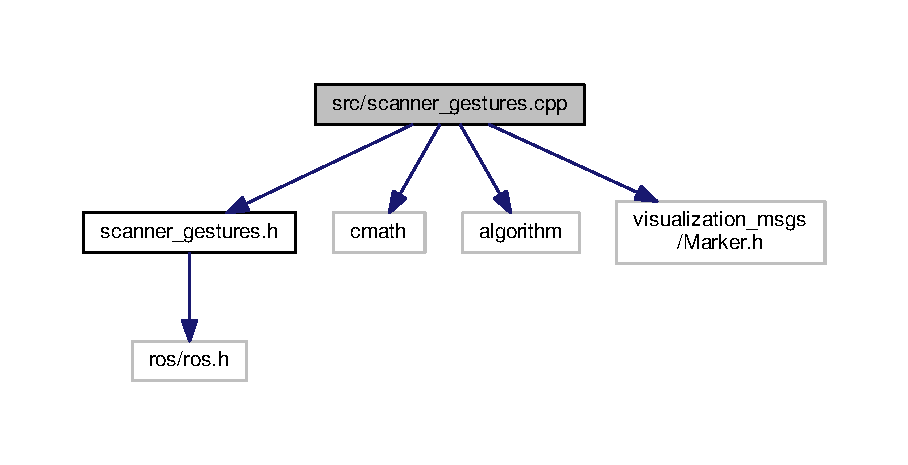
\includegraphics[width=350pt]{scanner__gestures_8cpp__incl}
\end{center}
\end{figure}

\hypertarget{track__objects__client_8cpp}{}\section{src/track\+\_\+objects\+\_\+client.cpp File Reference}
\label{track__objects__client_8cpp}\index{src/track\+\_\+objects\+\_\+client.\+cpp@{src/track\+\_\+objects\+\_\+client.\+cpp}}


R\+OS Client node of object tracker.  


{\ttfamily \#include \char`\"{}ros/ros.\+h\char`\"{}}\\*
{\ttfamily \#include \char`\"{}laser\+\_\+scanner\+\_\+infoscreen/track\+Objects.\+h\char`\"{}}\\*
{\ttfamily \#include \char`\"{}sensor\+\_\+msgs/\+Laser\+Scan.\+h\char`\"{}}\\*
{\ttfamily \#include \char`\"{}laser\+\_\+scanner\+\_\+infoscreen/biometrics.\+h\char`\"{}}\\*
{\ttfamily \#include \char`\"{}laser\+\_\+scanner\+\_\+infoscreen/biometrics\+\_\+results.\+h\char`\"{}}\\*
{\ttfamily \#include \char`\"{}laser\+\_\+scanner\+\_\+infoscreen/stepper\+\_\+control.\+h\char`\"{}}\\*
{\ttfamily \#include \char`\"{}laser\+\_\+scanner\+\_\+infoscreen/gesture\+\_\+call.\+h\char`\"{}}\\*
{\ttfamily \#include \char`\"{}laser\+\_\+scanner\+\_\+infoscreen/external\+\_\+control.\+h\char`\"{}}\\*
{\ttfamily \#include \char`\"{}std\+\_\+msgs/\+Int16.\+h\char`\"{}}\\*
{\ttfamily \#include $<$cstdlib$>$}\\*
{\ttfamily \#include $<$cmath$>$}\\*
{\ttfamily \#include $<$visualization\+\_\+msgs/\+Marker.\+h$>$}\\*
{\ttfamily \#include $<$string$>$}\\*
{\ttfamily \#include $<$chrono$>$}\\*
{\ttfamily \#include $<$thread$>$}\\*
Include dependency graph for track\+\_\+objects\+\_\+client.\+cpp\+:\nopagebreak
\begin{figure}[H]
\begin{center}
\leavevmode
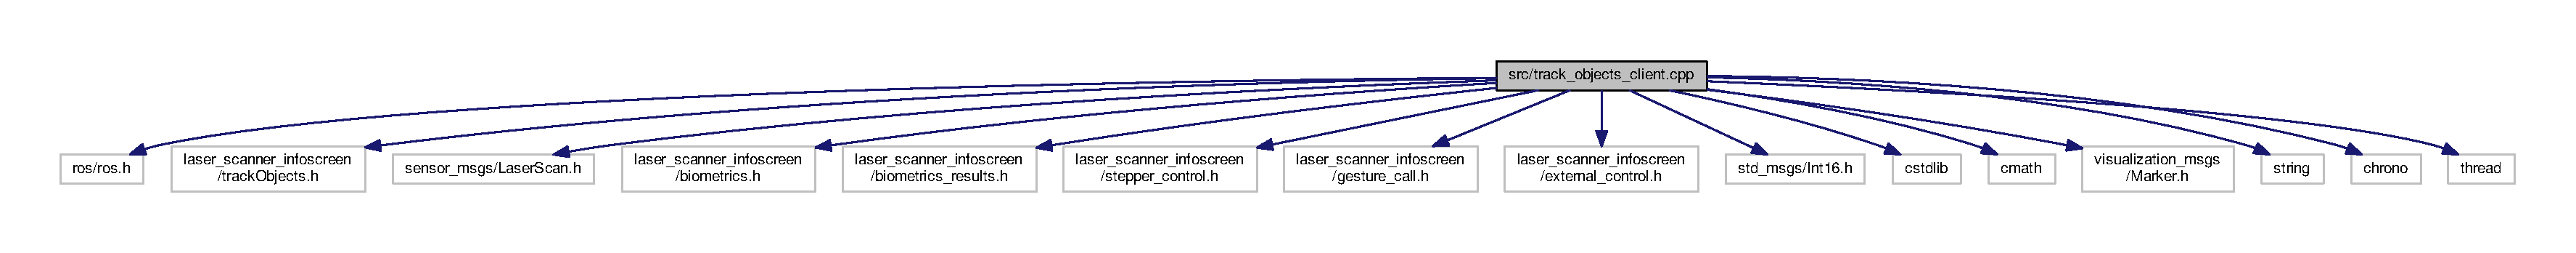
\includegraphics[width=350pt]{track__objects__client_8cpp__incl}
\end{center}
\end{figure}
\subsection*{Classes}
\begin{DoxyCompactItemize}
\item 
struct \hyperlink{structpoi__t}{poi\+\_\+t}
\begin{DoxyCompactList}\small\item\em Person of interest. \end{DoxyCompactList}\end{DoxyCompactItemize}


\subsection{Detailed Description}
R\+OS Client node of object tracker. 

Receives Laser\+Scan topic messages, passes them to the service, tracks the Person of Interest, and handles command of control of other nodes in the project.

\begin{DoxySeeAlso}{See also}
\hyperlink{track__objects__server_8cpp}{track\+\_\+objects\+\_\+server.\+cpp} 

laser\+\_\+objects 
\end{DoxySeeAlso}

\hypertarget{track__objects__server_8cpp}{}\section{src/track\+\_\+objects\+\_\+server.cpp File Reference}
\label{track__objects__server_8cpp}\index{src/track\+\_\+objects\+\_\+server.\+cpp@{src/track\+\_\+objects\+\_\+server.\+cpp}}


R\+OS Service node of object tracker.  


{\ttfamily \#include \char`\"{}ros/ros.\+h\char`\"{}}\\*
{\ttfamily \#include \char`\"{}laser\+\_\+scanner\+\_\+infoscreen/track\+Objects.\+h\char`\"{}}\\*
{\ttfamily \#include $<$visualization\+\_\+msgs/\+Marker.\+h$>$}\\*
{\ttfamily \#include $<$vector$>$}\\*
{\ttfamily \#include $<$cmath$>$}\\*
{\ttfamily \#include $<$utility$>$}\\*
{\ttfamily \#include $<$armadillo$>$}\\*
{\ttfamily \#include \char`\"{}laser\+\_\+objects.\+hpp\char`\"{}}\\*
Include dependency graph for track\+\_\+objects\+\_\+server.\+cpp\+:
\nopagebreak
\begin{figure}[H]
\begin{center}
\leavevmode
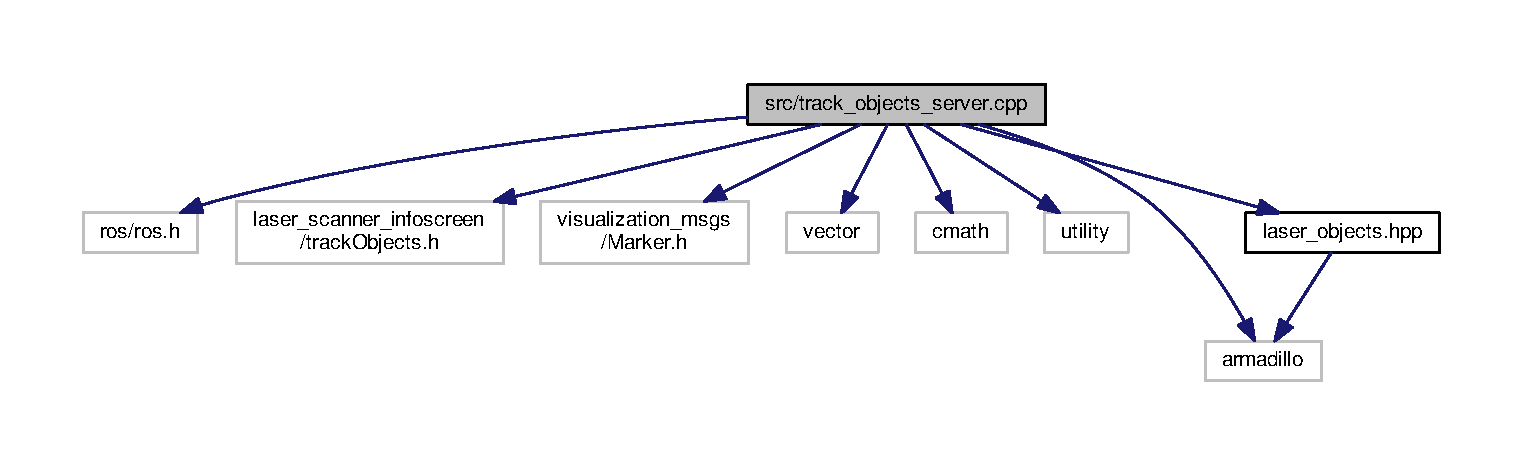
\includegraphics[width=350pt]{track__objects__server_8cpp__incl}
\end{center}
\end{figure}


\subsection{Detailed Description}
R\+OS Service node of object tracker. 

Handles low-\/level parsing Laser\+Scan message, and detecting and tracking objects. First culling is limiting wihtin 120deg cone to the front. Then points are broken into continuities of which between 0.\+4m and 0.\+7m long are passed to laser\+\_\+objects for further processing.

\begin{DoxySeeAlso}{See also}
\hyperlink{track__objects__client_8cpp}{track\+\_\+objects\+\_\+client.\+cpp} 

laser\+\_\+objects 
\end{DoxySeeAlso}

%--- End generated contents ---

% Index
\backmatter
\newpage
\phantomsection
\clearemptydoublepage
\addcontentsline{toc}{chapter}{Index}
\printindex

\end{document}
